\documentclass[a4]{article}
\usepackage{graphicx}
\usepackage{algorithm}
\usepackage{algorithmic}
\usepackage{lscape}
\usepackage{hyperref}
\usepackage{amssymb,longtable}
\usepackage[centertags]{amsmath}
\usepackage{amsfonts}
\usepackage{amsthm}
\usepackage{newlfont}
\usepackage{caption}
\usepackage{epsfig}
\newcommand{\norm}[1]{\left\Vert#1\right\Vert}

\textwidth  17.17cm
\textheight 23.4cm
\oddsidemargin -0.7mm
\evensidemargin -0.7mm
\def\baselinestretch{1.1}

\topmargin -8.4mm

\begin{document}

\title{Software Outlook: FFT Benchmarks for Fortran Codes }
\author{H. Sue Thorne}

\maketitle

%\begin{abstract}
%The abstract text goes here.
%\end{abstract}

\section{Introduction}
As part of the 2018/19 Software Outlook Work Plan, we will be benchmarking 
a number of different Fast Four Transform (FFT) libraries with bindings for
Fortran. The attributes of the different libraries are given in 
Section~\ref{Sec:libs}. Assuming indexing starts at 1, the discrete 1D Fourier transform of a vector $x$ of length $n$ is defined as
\begin{equation}\label{Eqn:fft}
  z(k) = \sum_{m=1}^{n} x(m) \exp(-2\pi i (k-1) (m-1) / n), \quad l=1,\ldots,n.
\end{equation}
In this work, we consider FFT libraries that have both multi-threading (OpenMP) and MPI capabilities.

\subsection{Half-complex format}
For input data that is purely real, the discrete Fourier transform satisfies 
the ``Hermitian'' redundancy: in 1D, if $x$ is a real array, then $z$ computed 
via (\ref{Eqn:fft}) will be a complex array satisfying
$$z(k) = \left[z(n-k+2)\right]^*, \quad k=2,\ldots,n.$$ Also note that the 
imaginary part of $z(1)$ is always 0; for $n$ even, the imaginary part of 
$z(n/2 + 1) $ is also always 0. This special symmetry in $z$ is known as 
\textit{half-complex} format and means that it can 
be stored more efficiently using a real array $y$ of length $n.$ The method of 
storing $z$ in $y$ will vary according to the library being used but one 
possibility is to define the values of $y$ as
\begin{eqnarray*}
y(1) & = & real(z(1)),\\
y(i) & = & real(z(i)), \quad i=2,\ldots,\lfloor n/2 \rfloor +1,\\
y(n-i+2) & = & imag(z(i)), \quad i=2,\ldots, \lfloor (n+1)/2  \rfloor.
\end{eqnarray*} 
Half-complex format can 
be extended to more dimensions. Note that if the input vector $x$ is 
half-complex format, then $z$ will be a real vector.

\section{Benchmarks}
\subsection{1D Benchmark}
Let $A$ be a 2D array with dimensions $n_1\times n_2$ and there be $q$ 
2D arrays $B_i$ that are the same size as $A.$  The general benchmark will take the form of 
Algorithm~\ref{Alg:1D}, where $comp\_mult(A,B_i)$ is defined to be 
component-wise multiplication of $A$ with $B_i;$  $comp\_div(H_i,B_i)$ 
is defined to be component-wise division of $H_i$ by $B_i;$ $\texttt{FFT}$ 
is the discrete Fast Fourier Transform and $\texttt{IFFT}$ is the 
discrete inverse Fast Fourier Transform.


\begin{algorithm}\caption{1D Benchmark}\label{Alg:1D}
\noindent \hrulefill

\begin{algorithmic}


\FOR {$i=1,\ldots,q$}

\STATE $C_i = comp\_mult(A,B_i)$

\FOR {$k=1,\ldots,n_2$}


\STATE $D_k = C_i(:,k)$

\STATE $F_k = \texttt{FFT}(D_k)$

\IF {do\_inverse}

\STATE $G_k = \texttt{IFFT}(F_k)$

\STATE $H(:,k) = G_k$

\ENDIF


\ENDFOR

\IF {do\_inverse}

\STATE $J_i = comp\_div(H_i,B_i) $

\STATE $abs\_err_i = \norm{A-J_i}_2$

\ENDIF

\ENDFOR

\end{algorithmic}
\noindent \hrulefill

\end{algorithm}

\subsection{2D Benchmark}
Let $A$ be a 3D array with dimensions $n_1\times n_2\times n_3$ and there be $q$ 
3D arrays $B_i$ that are the same size as $A.$  The benchmark will take the form of 
Algorithm~\ref{Alg:2D}, where $comp\_mult(A,B_i)$ is defined to be 
component-wise multiplication of $A$ with $B_i;$  $comp\_div(H_i,B_i)$ 
is defined to be component-wise division of $H_i$ by $B_i;$ $\texttt{FFT}$ 
is the discrete Fast Fourier Transform and $\texttt{IFFT}$ is the 
discrete inverse Fast Fourier Transform. This benchmark is designed to imitate 
some of the workload done in CCP\_PETMR's SIRF code.


\begin{algorithm}\caption{2D Benchmark}\label{Alg:2D}
\noindent \hrulefill

\begin{algorithmic}


\FOR {$i=1,\ldots,q$}

\STATE $C_i = comp\_mult(A,B_i)$

\FOR {$l=1,\ldots,n_3$}


\STATE $D_l = C_i(:,:,l)$

\STATE $F_l = \texttt{FFT}(D_l)$

\IF {do\_inverse}

\STATE $G_l = \texttt{IFFT}(F_l)$

\STATE $H(:,l) = G_l$

\ENDIF


\ENDFOR

\IF {do\_inverse}

\STATE $J_i = comp\_div(H_i,B_i) $

\STATE $abs\_err_i = \norm{A-J_i}_2$

\ENDIF

\ENDFOR

\end{algorithmic}
\noindent \hrulefill

\end{algorithm}

\subsection{3D Benchmark}
Let $A$ be a 3D array with dimensions $n_1\times n_2\times n_3$ and there be $q$ 
3D arrays $B_i$ that are the same size as $A.$  The benchmark will take the form of 
Algorithm~\ref{Alg:3D}, where $comp\_mult(A,B_i)$ is defined to be 
component-wise multiplication of $A$ with $B_i;$  $comp\_div(H_i,B_i)$ 
is defined to be component-wise division of $H_i$ by $B_i;$ $\texttt{FFT}$ 
is the discrete Fast Fourier Transform and $\texttt{IFFT}$ is the 
discrete inverse Fast Fourier Transform. 


\begin{algorithm}\caption{3D Benchmark}\label{Alg:3D}
\noindent \hrulefill

\begin{algorithmic}


\FOR {$i=1,\ldots,q$}

\STATE $C_i = comp\_mult(A,B_i)$



\STATE $F_i = \texttt{FFT}(C_i)$

\IF {do\_inverse}

\STATE $H_i = \texttt{IFFT}(F_i)$

\STATE $J_i = comp\_div(H_i,B_i) $

\STATE $abs\_err_i = \norm{A-J_i}_2$

\ENDIF

\ENDFOR

\end{algorithmic}
\noindent \hrulefill

\end{algorithm}

\section{FFT Libraries and testing environment}\label{Sec:libs}

In this work, we planned to compare the libraries listed in Table~\ref{Tbl:libs}. 
The datatypes listed are real (R), complex (C) and half-complex (H). The column 
"Dimensions" indicates the dimensions for which interfaces are provided. Lower 
dimensions can be input by calling the interface for higher dimensions and 
setting the dimension size to 1 for the additional dimensions.

\begin{table}[h]
\begin{center}
\begin{small}
\begin{tabular}{|l|c|c|c|l|l|c|}
\hline
\textbf{Library} & \textbf{Data types} & \textbf{Dimensions} & \textbf{Valid $n$} & \textbf{Parallelism} & \textbf{License} & \textbf{Citation} \\ \hline
FFTE & R $\rightarrow$ H & 2,3   & $2^a\times 3^b \times 5^c$ & OpenMP, MPI,  & Open source & \cite{FFTE} \\
     & C $\rightarrow$ C & 1,2,3 & & CUDA & & \\
     & H $\rightarrow$ R & 2,3   & & & & \\ \hline
FFTW & R $\rightarrow$ H & Any   & Any but optimised for  & Multithreading, & GPL v3 & \cite{FFTW} \\
     & C $\rightarrow$ C & Any      & $2^a\times 3^b\times 5^c\times 7^d\times 11^e\times 13^f$ &  MPI & & \\
     & H $\rightarrow$ R & Any      & with $e+f = 0$ or $1$ & & & \\ \hline
MKL  & R $\rightarrow$ H & Any   & Any & Multithreading, & Intel Simplified & \cite{MKL} \\
     & C $\rightarrow$ C & Any      & & MPI & Software License & \\
     & H $\rightarrow$ R & Any   & & & & \\ \hline
P3DFFT & R $\rightarrow$ H & 3   & Any & OpenMP, MPI & GPL v3 & \cite{P3DFFT} \\
     & H $\rightarrow$ R & 3   & & & & \\ \hline
%P3DFFT++ & R $\rightarrow$ H & 1,3   & Any & MPI & GPL v3 & \cite{P3DFFT} \\
%     & C $\rightarrow$ C &  1,3     & & &  & \\
%     & H $\rightarrow$ R & 1,3   & & & & \\ \hline

\end{tabular}
\caption{Libraries being benchmarked.  For ``valid $n$'', the values $a,$ $b,$ $c,$ $d,$ $e$ and $f$ are all assumed to be non-negative integers.}\label{Tbl:libs}
\end{small}
\end{center}
\end{table}

All benchmark runs were run on ARCHER **ADD REF**, where each compute node 
contains two 
2.7 GHz, 12-core E5-2697 v2 (Ivy Bridge) series processors. Each of the cores 
in these processors can support 2 hardware threads (Hyperthreads) but we do 
not activate hyperthreading within our benchmark tests. Within the node, the 
two processors are connected by two QuickPath Interconnect (QPI) links. All of 
our benchmarks were run on standard compute nodes, which have 64 GB of memory 
shared between the two processors. During our benchmark runs, we set the following environment variables:
\begin{itemize}
\item \texttt{KMP\_AFFINITY} to \texttt{disabled};
\item \texttt{OMP\_NUM\_THREADS} to the number of OpenMP threads;
\item \texttt{MKL\_NUM\_THREADS} to the number of OpenMP threads to ensure that the MKL runs use the full number of threads.
\end{itemize}
The benchmarks were launched via \texttt{aprun} with the flags set as 
\texttt{-cc none -n \$nprocs -d \$nthreads}, where \texttt{\$nprocs} is the 
number of MPI processes and \texttt{nthreads} is the number of OpenMP threads.

The default modules for  FFTW and Intel on ARCHER were used in our benchmarks, 
namely, versions 3.3.4.11 and 17.0.0.098, respectively. The Intel module 
contains MKL. FFTE was compiled using ARCHER's Intel Fortran compiler with flags \texttt{-O3 -fopenmp}. P3FFT version 2.7.9 was installed by following its installation instructions: the Intel compiler was used with the default Intel and FFTW modules; \texttt{configure} was called with the following flags:

\noindent \texttt{--prefix=[LOCAL] -enable-openmp}

\noindent \texttt{--enable-intel --enable-fftw --with-fftw=/opt/cray/fftw/default/ivybridge}

\noindent where \texttt{[LOCAL]} was set as a local directory.

[ADD INFO ABOUT wallclock, median value, accuracy checked, etc]


\section{1D Real results}


In this section we discuss the benchmark results for libraries that apply the 
fast Fourier transform to real 1D arrays. The numerical results from the FFTE 
library were found to be inaccurate and, whilst it was straightforward to 
debug the code, we are testing the codes as provided so we exclude this 
library from these benchmarks. The P3DFFT library cannot be used on 1D 
problems and, hence, is excluded.

In these benchmarks, we set $n_2=4$ and $n_q=4.$ For one set of tests, we let
 $n_1=2^k$ for $k=8,\ldots,30.$ For the other set of tests, $n_1$ is defined 
to be the closest prime number to $2^k,$ $k=8,\ldots,20:$ if two primes are 
equidistant, we choose the larger one.

We start by considering the MPI-OpenMP versions of the FFTW and MKL libraries.

\subsection{FFTW}

 In Figure~\ref{Fig:fftw1d_times}, we compare single node experiments for FFTW with 1, 8 and 16 
MPI processes but fix the number of OpenMP threads to 1. We provide both the 
initialisation time ``INIT'' for the FFT library call and the FFT computation 
time ``FFT''. For values of $n_1$ that are powers of 2, we could only perform 
computations up to $2^14$ due to the Fortran to C interface relying on 
C\_INTPTR\_T, which, on ARCHER, has size 4 bytes. As a result, the problem size, 
$n_1,$ is not large enough to allow the MPI capabilities to affect. For the 
larger values of $n_1,$ we note that when $n_1$ is prime, the 
initialisation time between one and two orders of magnitude larger than when $n_1$ was a power of 2; the FFT computation time is roughly an order of magnitude 
larger than when $n_1$ switches from beinga power of 2 to being prime. Additionally, for prime values of $n_1,$ the initialisation time is between 4 and 5 orders of magnitude larger than the FFT computation time. For values of $n_1$ that are powers of 2 but smaller than 10000, the FFT computation time is smallest when just one  MPI process is used but this is sometimes countered by an increase in the intialisation time.

\begin{figure}[!htbp]
\begin{center}
 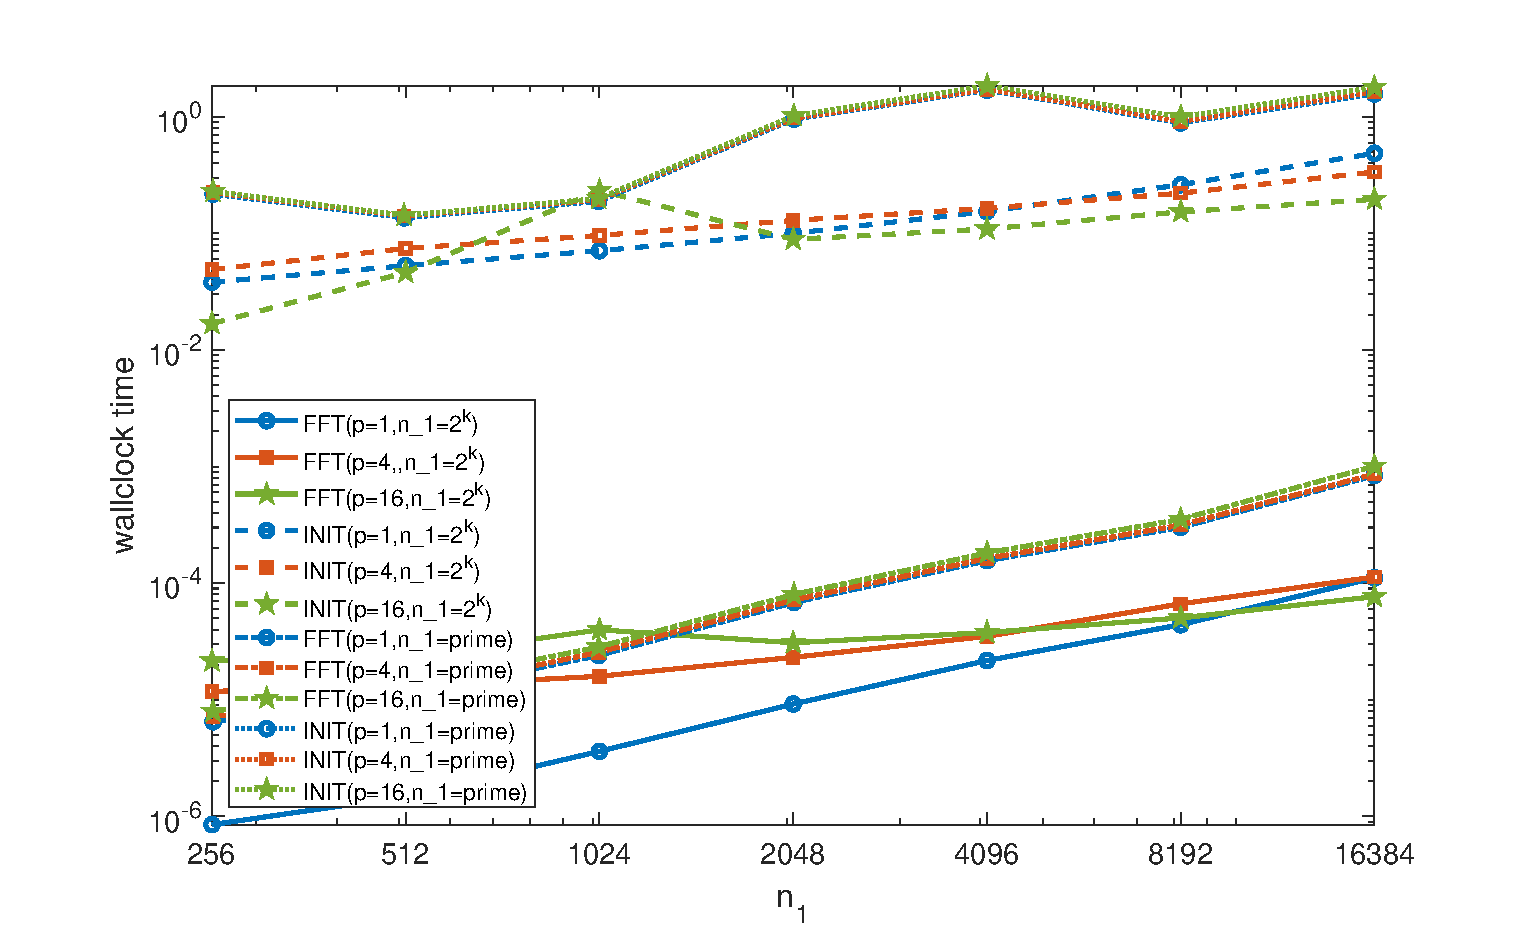
\includegraphics[width=.9\textwidth, height=0.42\textheight]{FFTW1D_times_fig.eps}
\caption{1D FFTW applied to real valued one-dimensional arrays of length $n_1$ using $p$ MPI processes. Wallclock initialisation time, INIT, and wallclock FFT time, FFT, are given in seconds.}
\label{Fig:fftw1d_times}
\end{center}
\end{figure}



In Figure~\ref{Fig:fftw1d_threads_times} we fix the number of MPI processes to one and vary the number of OpenMP threads. As with the tests where the number of threads was fixed at one and the number of MPI threads were varied, the problem sizes considered do not see any benefit from using multiple threads until we reach $n_1=16384$ (16381 in the prime tests). 


\begin{figure}[!htbp]
\begin{center}
 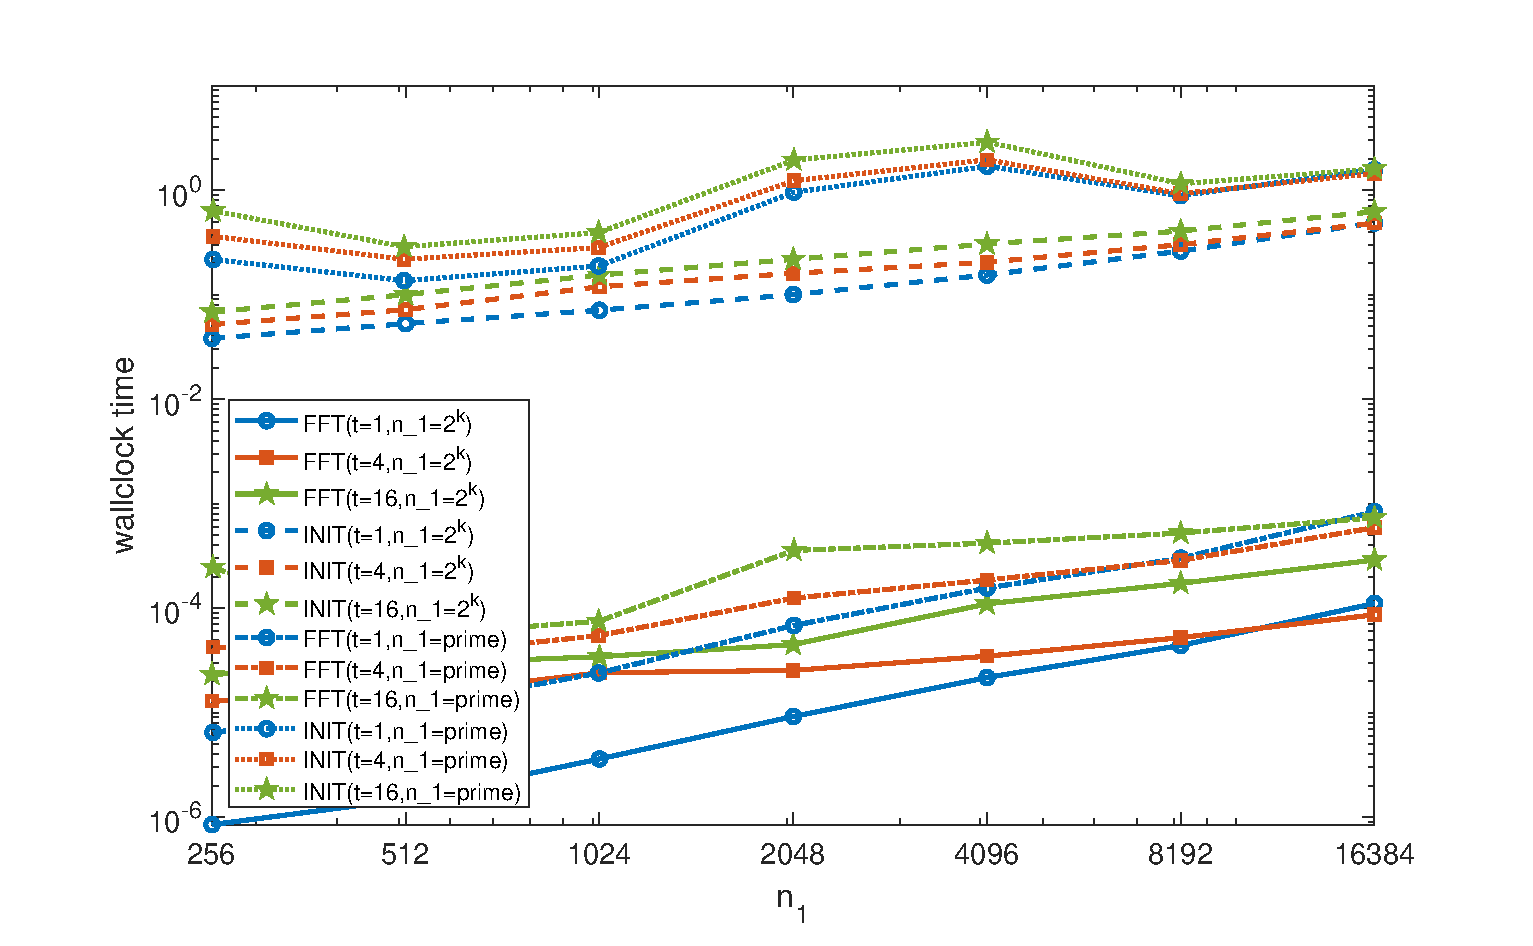
\includegraphics[width=.9\textwidth, height=0.42\textheight]{FFTW1D_threads_times_fig.eps}
\caption{1D FFTW applied to real valued one-dimensional arrays of length $n_1$ using $t$ threads and 1 MPI process. Wallclock initialisation time, INIT, and wallclock FFT time, FFT, are given in seconds.}
\label{Fig:fftw1d_threads_times}
\end{center}
\end{figure}




In Tables~\ref{Tbl:FFT1d2048}, \ref{Tbl:FFT1d2053}, \ref{Tbl:FFT1d16381} and \ref{Tbl:FFT1d16384},  the FFT compution and initialisation wallclock times and ratios with respect to 1 MPI process combined with 1 OpenMP thread are provided for $n_1=2048,$ $n_1=2053,$  $n_1=16381$ and  $n_1=16384,$ respectively.




\begin{table}
\begin{center}
%\being{small}
\begin{tabular}{|r|r|r|r|r|r|r|r|r|}
\hline 
     &  & \multicolumn{7}{c|}{$t$} \\ \hline
    $p$  &  & 1           & 2    & 4    & 8    & 12   & 16    & 24  \\ \hline\hline
    1  & ftime & 9.19e-6 & 2.05e-5 & 2.54e-5 &  2.81e-5 &   4.03e-5 &   4.49e-5 &  1.84e-4 \\ 
      & fratio & 1.0 & 2.23 & 2.76 &  3.06 &   4.39 &  4.89 &  20.0 \\ 
     & itime &  1.00e-1 &   1.18e-1 &   1.60e-1 &   1.96e-1 &   2.53e-1 &   2.18e-1 &   2.79e-1   \\ 
     & iratio &  1.00 &    1.18 &    1.60 &    1.96 &    2.53 &    2.18 &    2.79   \\ \hline
    2  & ftime & 3.05e-5 &  6.39e-5 &  8.63e-5 &  1.08e-4 &  3.95e-4 & - & - \\ 
      & fratio & 3.32 &  6.95 &  9.39 &  11.8 &   43.0 &  &  \\
      & itime &   1.55e-1 &   2.24e-1 &   2.96e-1 &   3.21e-1 &   4.82e-1   &  &  \\
      & iratio &  1.55 &    2.24 &    2.96 &    3.21 &    4.82    &  &  \\ \hline
    4  & ftime &  2.31e-5 &  7.10e-5  & 8.35e-5 & - & - & - & - \\ 
      & fratio & 2.51 &  7.73  & 9.09 &  &  &  &  \\
      & itime &   1.29e-1 &   1.91e-1 &   2.04e-1    &  & & & \\
      & iratio &  1.29 &    1.91 &    2.04    &  & & &  \\ \hline
    8  & ftime & 2.78e-5 &  8.17e-05 & - & - & - & - & - \\ 
      & fratio & 3.03 &  8.89 &  &  &  &  &  \\
      & itime &   1.04e-1 &   1.56e-1    &  & & & & \\
      & iratio & 1.04 &    1.56    &  & & & & \\ \hline
    16 & ftime  & 3.08e-5 & - & - & - & - & - & - \\ 
     & fratio & 3.35 &  &  &  &  &  &  \\
      & itime &   8.87e-2   & & & & & & \\
      & iratio &   0.89  & & & & & & \\ \hline
\end{tabular}
\caption{1D FFTW applied to real valued one-dimensional arrays of length $n_1=2048$ using $p$ MPI processes and $t$ threads. The wallclock FFT computation time, ftime, (in seconds); the ratio, fratio, of ftime  with ftime($p=1,t=1$); wallclock FFT initialisation time, itime, (in seconds); the ratio, iratio, of itime  with itime($p=1,t=1$) are provided.}\label{Tbl:FFT1d2048}
%\end{small}
\end{center}
\end{table}



\begin{table}
\begin{center}
%\being{small}
\begin{tabular}{|r|r|r|r|r|r|r|r|r|}
\hline 
     &  & \multicolumn{7}{c|}{$t$} \\ \hline
    $p$  &  & 1           & 2    & 4    & 8    & 12   & 16    & 24  \\ \hline\hline
    1  & ftime & 6.84e-5 &  9.10e-5 &  1.25e-4 &  1.66e-4 &  2.91e-4 &  3.57e-4 &  8.80e-4  \\ 
      & fratio & 1.00 &    1.33 &    1.83 &    2.43 &    4.25 &    5.22 &    12.9 \\
     & itime & 9.55e-1 &   9.95e-1 &   1.23e0 &   1.47e0 &   1.79e0 &   1.94e0 &   2.33e0 \\ 
     & iratio & 1.00 &   1.04 &   1.29 &   1.54 &   1.87 &   2.03 &   2.44   \\  \hline
    2  & ftime & 6.89e-5 &  9.29e-5 &  1.34e-4 &  1.69e-4 &  5.52e-4  & - & - \\ 
      & fratio &  1.01 &    1.36 &    1.96 &    2.47 &    8.07     &  &  \\
      & itime &  9.67e-1 &   1.03e0 &   1.24e0 &   1.49e0 &   1.80e0  &  &  \\
      & iratio &  1.01 &   1.08 &   1.30 &   1.56 &   1.88  &  &  \\ \hline
    4  & ftime & 7.17e-5 &  9.96e-5 &  1.33e-4  & - & - & - & - \\ 
      & fratio &  1.05 &    1.46 &    1.94    &  &  &  &  \\
      & itime &  9.73e-1 &   1.03e0 &   1.23e0   &  & & & \\
      & iratio & 1.02 &   1.08 &   1.29   &  & & &  \\ \hline
    8  & ftime &7.62e-5 &  1.02e-4  & - & - & - & - & - \\ 
      & fratio & 1.11 &    1.49    &  &  &  &  &  \\
      & itime &  1.00e0 &   1.04e0  &  & & & & \\
      & iratio &  1.05 &   1.09   &  & & & & \\ \hline
    16 & ftime  &    8.00e-5  & - & - & - & - & - & - \\ 
     & fratio &     1.17   &  &  &  &  &  &  \\
      & itime & 1.02e0   & & & & & & \\
      & iratio & 1.07  & & & & & & \\ \hline
\end{tabular}
\caption{1D FFTW applied to real valued one-dimensional arrays of length $n_1=2053$ using $p$ MPI processes and $t$ threads. The wallclock FFT computation time, ftime, (in seconds); the ratio, fratio, of ftime  with ftime($p=1,t=1$); wallclock FFT initialisation time, itime, (in seconds); the ratio, iratio, of itime  with itime($p=1,t=1$) are provided. }\label{Tbl:FFT1d2053}
%\end{small}
\end{center}
\end{table}


\begin{table}
\begin{center}
%\being{small}
\begin{tabular}{|r|r|r|r|r|r|r|r|r|}
\hline 
     &  & \multicolumn{7}{c|}{$t$} \\ \hline
    $p$  &  & 1           & 2    & 4    & 8    & 12   & 16    & 24  \\ \hline\hline
    1  & ftime &  8.38e-4 &  6.01e-4 &  5.90e-4 &  5.89e-4 &  7.43e-4 &  7.33e-4 &  9.93e-4  \\ 
      & fratio & 1.00 &  0.72 &  0.70 &  0.70 &  0.89 &  0.87 &  1.19   \\ 
     & itime & 1.57e0 &   1.55e0 &   1.45e0 &   1.50e0 &   1.59e0 &   1.60e0 &   1.84e0  \\ 
     & iratio & 1.00 &   0.99 &   0.92 &   0.96 &   1.01 &   1.02 &   1.17  \\ \hline
    2  & ftime &  7.96e-4 &  6.49e-4 &  6.32e-4 &  6.08e-4 &  8.62e-4  & - & - \\ 
      & fratio &   0.95 &  0.77 &  0.75 &  0.73 &  1.03   &  &  \\
      & itime &  1.59e0 &   1.57e0 &   1.48e0 &   1.49e0 &   1.64e0   &  &  \\
      & iratio &  1.01 &   1.00 &   0.94 &   0.95 &   1.04  &  &  \\ \hline
    4  & ftime & 8.62e-4 &  6.67e-4 &  6.03e-4   & - & - & - & - \\ 
      & fratio &   1.03 &  0.80 &  0.72  &  &  &  &  \\
      & itime &  1.63e0 &   1.57e0 &   1.51e0   &  & & & \\
      & iratio &  1.03 &   1.00 &   0.96  &  & & &  \\ \hline
    8  & ftime &  8.40e-4 &  6.99e-4    & - & - & - & - & - \\ 
      & fratio & 1.00 &  0.83  &  &  &  &  &  \\
      & itime &  1.71e0 &   1.70e0   &  & & & & \\
      & iratio &  1.09 &   1.08  &  & & & & \\ \hline
    16 & ftime  & 1.01e-3    & - & - & - & - & - & - \\ 
     & fratio &  1.21   &  &  &  &  &  &  \\
      & itime &   1.79e0  & & & & & & \\
      & iratio & 1.14   & & & & & & \\ \hline
\end{tabular}
\caption{1D FFTW applied to real valued one-dimensional arrays of length $n_1=16381$ using $p$ MPI processes and $t$ threads. The wallclock FFT computation time, ftime, (in seconds); the ratio, fratio, of ftime  with ftime($p=1,t=1$); wallclock FFT initialisation time, itime, (in seconds); the ratio, iratio, of itime  with itime($p=1,t=1$) are provided. }\label{Tbl:FFT1d16381}
%\end{small}
\end{center}
\end{table}

\begin{table}
\begin{center}
%\being{small}
\begin{tabular}{|r|r|r|r|r|r|r|r|r|}
\hline 
     &  & \multicolumn{7}{c|}{$t$} \\ \hline
    $p$  &  & 1           & 2    & 4    & 8    & 12   & 16    & 24  \\ \hline\hline
    1  & ftime &   1.11e-4 &  9.20e-5 &  8.65e-5 &  7.81e-5 &  3.35e-4&   2.89e-4 &  5.16e-4  \\ 
      & fratio & 1.0000 &   0.83 &   0.78 &   0.70 &   3.02 &   2.60 &   4.65   \\
     & itime & 4.86e-1 &   4.82e-1 &   4.84e-1 &   5.41e-1 &   6.23e-1 &   6.21e-1 &   7.27e-1  \\ 
     & iratio &  1.0000 &   0.99 &  1.00 &   1.11 &   1.28 &   1.28 &   1.50  \\  \hline
    2  & ftime & 1.93e-4  & 2.51e-4 &  2.88e-4 &  3.27e-4 &  8.46e-4  & - & - \\ 
      & fratio &   1.74 &   2.26 &   2.59 &   2.95 &   7.62    &  &  \\
      & itime &     5.10e-1 &   6.58e-1 &   9.09e-1 &   1.02e0 &   1.43e0   &  &  \\
      & iratio & 1.05 &   1.35 &   1.87 &   2.10 &   2.94   &  &  \\ \hline
    4  & ftime &  1.13e-4 &  1.94e-4 &  3.46e-4 & - & - & - & - \\ 
      & fratio &   1.02 &   1.75 &   3.12   &  &  &  &  \\ 
      & itime &   3.36e-1 &   4.64e-1 &   5.18e-1  &  & & & \\
      & iratio & 0.69 &   0.95 &   1.07   &  & & &  \\\hline
    8  & ftime & 8.44e-5 &  1.66e-4   & - & - & - & - & - \\ 
      & fratio &  0.76 &   1.50   &  &  &  &  &  \\
      & itime &  2.34e-1 &   3.53e-1   &  & & & & \\
      & iratio &  0.48 &   0.73  &  & & & & \\ \hline
    16 & ftime  &  7.66e-5   & - & - & - & - & - & - \\ 
     & fratio &    0.69  &  &  &  &  &  &  \\
      & itime &  1.96e-1   & & & & & & \\
      & iratio & 0.40   & & & & & & \\ \hline
\end{tabular}
\caption{1D FFTW applied to real valued one-dimensional arrays of length $n_1=16384$ using $p$ MPI processes and $t$ threads. The wallclock FFT computation time, ftime, (in seconds); the ratio, fratio, of ftime  with ftime($p=1,t=1$); wallclock FFT initialisation time, itime, (in seconds); the ratio, iratio, of itime  with itime($p=1,t=1$) are provided. }\label{Tbl:FFT1d16384}
%\end{small}
\end{center}
\end{table}









\bibliographystyle{siam}
\bibliography{bib2017}


\end{document}
